\documentclass[11pt]{article}
\usepackage[margin=0.9in]{geometry}
\usepackage[dvipsnames]{xcolor}
\usepackage{graphicx,booktabs,amsmath,amssymb,hyperref,caption,placeins,enumitem,tikz}
\usetikzlibrary{arrows.meta,positioning,calc,fit,decorations.pathreplacing}
\usepackage[T1]{fontenc}
\captionsetup{font=small,labelfont=bf}
\hypersetup{colorlinks=true,linkcolor=blue!50!black,urlcolor=blue!50!black,citecolor=blue!50!black}
\setlist{itemsep=1pt,topsep=2pt}
\newcommand{\nmse}{\mathrm{nMSE}}
\newcommand{\dx}{\partial_x}
\newcommand{\fig}[3][\textwidth]{\begin{figure}[htbp]\centering\IfFileExists{figs/#2.png}{\includegraphics[width=#1]{figs/#2.png}}{\fbox{\parbox{0.9\textwidth}{\centering figure #2 not yet made}}}\caption{#3}\label{fig:#2}\end{figure}}

\title{An ordered latent field for a cloud-resolving squall line,\\and what a PDE for its leading channel says}
\author{}
\date{9 November 2026}

\begin{document}
\maketitle

\begin{abstract}
We emulate two-dimensional CM1 squall lines with a \emph{local} latent model: each 2\,km patch of the domain becomes a site carrying 32 latent channels, and a stencil law advances the field one minute at a time. Training windows are centred on the storm half of the time, and a structured (nested) dropout orders the channels by importance, so that channel~0 alone reconstructs the full 434-variable column state to $\nmse = 0.30$, where an ordinary latent needs about 12 channels. Channel~0 is a cold-pool/convection coordinate. Sparse regression on it finds that its evolution is transport, not local growth: a law with spatial derivatives explains 21--42\% of its held-out tendency from channel~0 alone, a local ODE explains nothing. Rewritten in physical units through a fixed map to surface $\theta'$, the leading law is an advection whose speed is linear in the cold-pool temperature deficit, $c(\theta') = 0.20 + 0.049\,\theta'$\,km\,min$^{-1}$, with a tight and test-reproducible slope, and an anti-diffusive term. Its speed at the gust front matches the measured cold-pool speed on average, and a second, independently trained autoencoder gives the same law within about 20\%. Two pre-registered tests of physical meaning fail, however: the speed does not track storm-to-storm differences, and its dependence on $\theta'$ is 3.5$\times$ steeper than density-current scaling.
\end{abstract}

\section{Data and model}\label{sec:model}
\paragraph{Data.} CM1 r21.1 two-dimensional ($x$--$z$) squall lines, 400\,km wide with $\Delta x = 250$\,m, 62 stretched levels, open lateral boundaries and a grid moving at 12.5\,m\,s$^{-1}$; Morrison two-moment microphysics; 6\,h runs with 1-min output. 121 storms from three ensembles (control sounding with random initial noise; and boundary-layer moisture $\times$ wind-shear variations), split by storm into training, validation and test sets. Each column holds 7 variables ($u'$, $w$, $\theta'$, $q_v'$, $p'$, $\sqrt{q_\mathrm{liq}}$, $\sqrt{q_\mathrm{ice}}$) on 62 levels, as perturbations from the far-field initial column, standardized per variable: 434 numbers per grid column, 1\,600 columns.

\paragraph{Channels and patches.} The autoencoder is a 1D convolution along $x$ with the column as the channel dimension (Fig.~\ref{fig:schematic}):
\begin{itemize}
\item \textbf{Patchify}: a convolution with kernel = stride = 8 maps each 8-column patch (2\,km) to a hidden vector of width 256. The domain becomes $P = 200$ \emph{sites}.
\item \textbf{Mix}: two residual convolutions of radius 1 along the sites, so each site sees $\pm 2$ neighbouring sites ($\pm4$\,km); no circular padding (the boundaries are open).
\item \textbf{Project}: a $1\times1$ convolution without bias to $c = 32$ latent channels per site.
\end{itemize}
The latent state is therefore a \emph{field} $z_j(t) \in \mathbb{R}^{32}$, $j = 1..200$, not a single vector. Shifting the input by a whole patch shifts the latent by one site. The decoder mirrors the encoder (transposed convolution, kernel = stride = 8).

\paragraph{Propagator: an explicit latent PDE.} The model used here advances the field with a local law, one frame (1\,min) per step, integrated with a Heun step:
\begin{equation}
\partial_t z = A_0 z + A_1 \dx z + A_2 \partial_x^2 z + b + Q_1[z_i z_j] + Q_2[z_i\, \dx z_j] + R(z, \dx z, \partial_x^2 z),
\label{eq:law}
\end{equation}
with centred differences over sites, a small pointwise MLP residual $R$, and a soft tendency cap. All coefficients start at zero (identity step). The residual ends up carrying only 1--3\% of the tendency, so this 32-channel law forecasts CM1 as well as a neural stencil network. But it is dense: tens of thousands of its 52\,736 coefficients are needed, and no readable law can be pruned from it. That is the motivation for Section~\ref{sec:pde}: ask for a short law for the \emph{leading} channels of an \emph{ordered} latent instead.

\paragraph{Training.} Stage A trains the autoencoder (reconstruction, plus a log-determinant term against channel collapse). Stage B trains the propagator on latent rollouts of up to 45 steps with the autoencoder frozen. Stage C fine-tunes both jointly on decoded 45-step rollouts, with the 3-site halo of every window forced by the true state.

\begin{figure}[htbp]\centering
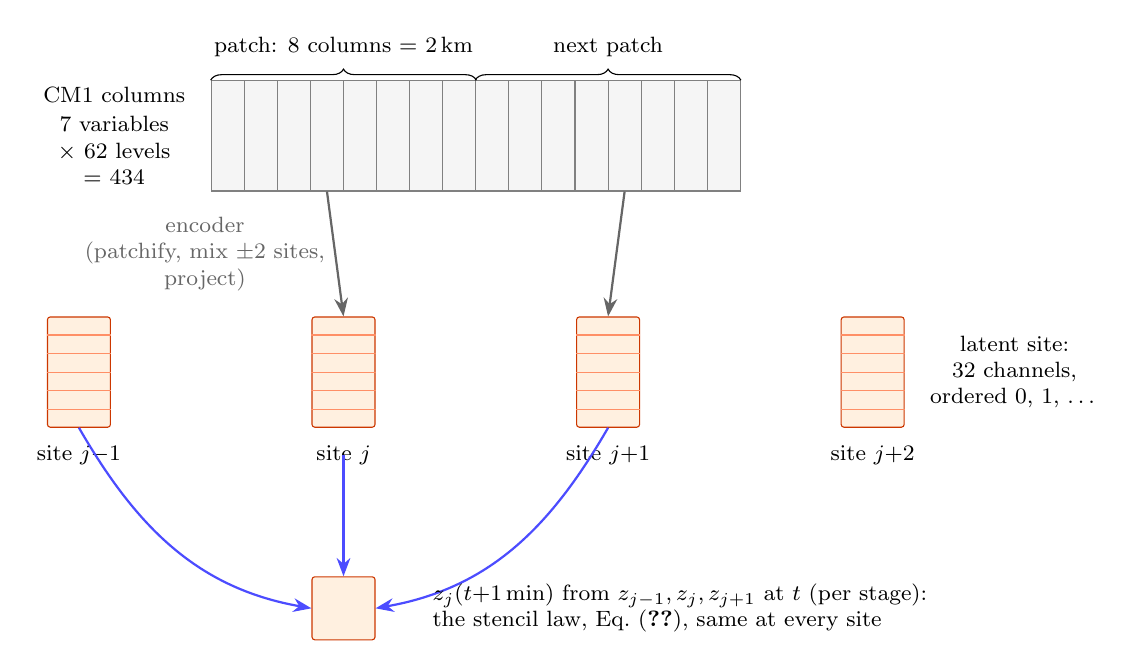
\begin{tikzpicture}[font=\small, >=Stealth,
  cell/.style={draw=black!50, fill=black!4, minimum width=4.2mm, minimum height=14mm, inner sep=0},
  site/.style={draw=OrangeRed!80!black, fill=orange!12, minimum width=8mm, minimum height=14mm, inner sep=0, rounded corners=1pt},
  lab/.style={align=center, font=\footnotesize}]
  % columns
  \foreach \i in {0,...,15} {\node[cell] (c\i) at (\i*0.42, 0) {};}
  \draw[decorate,decoration={brace,amplitude=4pt}] (c0.north west) -- (c7.north east) node[midway, above=5pt, lab] {patch: 8 columns = 2\,km};
  \draw[decorate,decoration={brace,amplitude=4pt}] (c8.north west) -- (c15.north east) node[midway, above=5pt, lab] {next patch};
  \node[lab, left=2mm of c0] {CM1 columns\\[1pt]7 variables\\$\times$ 62 levels\\= 434};
  % sites
  \node[site] (s0) at (1.47, -3.0) {}; \node[site] (s1) at (4.83, -3.0) {};
  \node[site] (sm) at (-1.89, -3.0) {}; \node[site] (sp) at (8.19, -3.0) {};
  \foreach \s in {s0,s1,sm,sp} {\foreach \k in {1,...,5} {\draw[OrangeRed!60] ($(\s.north west)!{\k/6}!(\s.south west)$) -- ($(\s.north east)!{\k/6}!(\s.south east)$);}}
  \draw[->, thick, black!60] (c3.south) -- (s0.north) node[midway, left, lab] {encoder\\(patchify, mix $\pm$2 sites,\\project)};
  \draw[->, thick, black!60] (c12.south) -- (s1.north);
  \node[lab, right=2mm of sp] {latent site:\\32 channels,\\ordered 0, 1, \dots};
  \node[lab, below=1mm of s0] {site $j$}; \node[lab, below=1mm of s1] {site $j{+}1$};
  \node[lab, below=1mm of sm] {site $j{-}1$}; \node[lab, below=1mm of sp] {site $j{+}2$};
  % stencil
  \node[site, minimum height=8mm] (n0) at (1.47, -6.0) {};
  \draw[->, thick, Blue!70] (sm.south) to[out=-60,in=170] (n0.west);
  \draw[->, thick, Blue!70] (s0.south) ++(0,-0.35) -- (n0.north);
  \draw[->, thick, Blue!70] (s1.south) to[out=-120,in=10] (n0.east);
  \node[lab, right=6mm of n0, text width=7.5cm, align=left] {$z_j(t{+}1\,\mathrm{min})$ from $z_{j-1}, z_j, z_{j+1}$ at $t$ (per stage):\\the stencil law, Eq.~(\ref{eq:law}), same at every site};
\end{tikzpicture}
\caption{The local latent model. Each 2\,km patch of CM1 columns is encoded into one site with 32 channels; nested dropout orders them so that channel~0 carries most of the column. A shared stencil law advances every site from its neighbours.}\label{fig:schematic}
\end{figure}

\section{Storm-centred training}\label{sec:storm}
Most of the 400\,km domain is quiet environment most of the time: a squall line occupies a few tens of kilometres. Uniformly sampled windows would spend most of the training signal on near-zero perturbations. Every stage therefore draws half of its training windows ($\texttt{active\_frac} = 0.5$) centred on a storm column, a randomly chosen grid column and time with composite reflectivity above 10\,dBZ; the other half is drawn uniformly, so the quiet environment and the storm's surroundings are still learned (Fig.~\ref{fig:fig_sampling}). Windows are 32 sites (64\,km) for the autoencoder, 48 sites (96\,km) $\times$ up to 47 frames for the propagator. Because the model is local, a window is a complete training example: the same weights are applied to the whole 200-site domain at test time.
\fig[0.85\textwidth]{fig_sampling}{Composite reflectivity of one training storm (grey) with six storm-centred (left) and six uniform (right) Stage~B windows. Half of all windows are storm-centred; the uniform half covers the environment.}

\section{Structured (nested) dropout: an ordered latent}\label{sec:nested}
In an ordinary autoencoder the 32 channels are interchangeable: any rotation of the latent is equally good, so no single channel means anything. Nested dropout breaks this symmetry. For half of the training samples, an integer $k$ is drawn uniformly from $1..32$, channels $k..31$ are set to zero, and the decoder must reconstruct the column from channels $0..k{-}1$ alone. Channel~0 is then trained to be the best one-channel description of the column, channels 0--1 the best pair, and so on: a nonlinear analogue of a principal-component ordering. The truncation acts on the reconstruction terms of Stage~A and Stage~C; the propagator always sees all channels.

The ordering is strong (Fig.~\ref{fig:fig_ordering}): channel~0 alone reconstructs the column to $\nmse = 0.30$, and 4 channels to 0.14. The ordinary latent needs about 12 channels to reach 0.5 with its first channels. With all 32 channels the two latents reconstruct about equally well (0.031 against 0.026), so the ordering costs little. A second nested autoencoder trained from scratch with a different seed gives the same curve to within 0.01.
\fig[0.6\textwidth]{fig_ordering}{Reconstruction error with only the first $k$ channels kept (others set to zero), on unseen test storms. Nested dropout orders the channels by importance; the ordinary latent spreads information evenly.}

\paragraph{What channel 0 is.} On the test storms, channel~0 correlates $+0.80$ with surface $\theta'$, $-0.86$ with column condensate, $-0.72$ with column-maximum $w$ and $-0.46$ with low-level $u'$ (site means). Decoding a field in which only channel~0 is set shows what it encodes (Fig.~\ref{fig:fig_channel0_profiles}): negative values are a mature convective column, with a surface cold pool of $-8$\,K, latent warming aloft, liquid water below the melting level and an ice anvil above, and a reversal of $u'$ with height (low- and mid-level flows of opposite sign, $\sim$10\,m\,s$^{-1}$). Positive values are the undisturbed environment. In space and time (Fig.~\ref{fig:fig_hovmoller_law}, first two panels) channel~0 tracks the cold pool and the gust front. It is a cold-pool/convection coordinate. Channels 1--3 have no comparably clear physical correlate ($|r| \le 0.46$).
\fig{fig_channel0_profiles}{Decoded column at a site when only channel~0 is non-zero, for four values of $z_0$; the surface $\theta'$ each value maps to (Sec.~\ref{sec:units}) is in the legend. Condensate is plotted as $\sqrt{q}$ (g\,kg$^{-1}$)$^{1/2}$.}

\section{Interpretable PDEs for the leading channels}\label{sec:pde}
\paragraph{Method.} For the first $k$ channels of the ordered latent ($k = 1, 2, 4, 8$) we fit $\partial_t z_j$ (centred difference, per minute) for $j < k$ by bootstrap sequentially thresholded least squares (STLSQ, resampling whole storms) on 30 training storms, frames 30--330\,min, and score on 10 test storms. The candidate libraries are built from the first $k$ channels only:
\begin{itemize}
\item \textbf{local ODE}: $z$ and quadratic products (no neighbours);
\item \textbf{PDE}: plus $\dx z$, $\partial_x^2 z$ (and optionally up to $\partial_x^4 z$) and their products with $z$;
\item options: products of two derivatives (KPZ-type), cubic terms, second order in time, and a BBM-type mixed operator $(1 - \ell^2\partial_x^2)\partial_t z$.
\end{itemize}
Coefficients are in sites (2\,km) and minutes. Decision rules for each test were written down before the corresponding run.

\paragraph{Channel 0 is transported, not locally driven.} Fig.~\ref{fig:fig_r2_vs_k} shows the held-out $R^2$ of channel~0's tendency. A local ODE explains essentially nothing at any $k$ ($R^2 \le 0.2$); spatial derivatives explain 21\% from channel~0 alone (42\% with third and fourth derivatives), rising to 56--61\% with two channels and 76--82\% with eight. On the ordinary (unordered) latent the same procedure finds almost nothing ($R^2 \le 0.27$): the ordering is what makes a leading-channel law possible.
\fig[0.6\textwidth]{fig_r2_vs_k}{Held-out $R^2$ of channel~0's tendency against the number of channels in the law (threshold 0.03). Orange/green: ordered latent; blue: ordinary latent. Dotted: local ODE; solid: with spatial derivatives.}

\paragraph{The shortest laws.} With channel~0 alone, the sparsest PDE (3 terms) is a nonlinear advection,
\begin{equation}
\partial_t z_0 = -(0.059 + 0.082\, z_0)\, \dx z_0 - 0.004 .
\label{eq:adv}
\end{equation}
With more channels, channel~0's equation keeps the same form, but its advecting velocity is built from several channels: for $k = 8$ its 13 terms are almost all of the form $z_i\, \dx z_j$, led by
$\partial_t z_0 \approx (0.069\, z_1 - 0.064\, z_0)\, \dx z_0 - 0.050\, z_1 \dx z_1 + \dots$ (Table~\ref{tab:terms}). The selected structure is stable across bootstrap resamples. Other library extensions add little: a $(\dx z_0)^2$ term (KPZ-type) is selected with a consistently negative sign; cubic terms and second order in time do not help; third-derivative terms raise $R^2$ but their coefficient doubles when the field is smoothed by one more site, so they describe the unresolved sharpness of the gust front rather than a physical dispersion.

\begin{table}[htbp]\centering\small
\caption{Selected terms of channel~0's equation (one-step fit, threshold 0.1; coefficients in sites and minutes; bootstrap selection frequency 1.0 unless noted).}\label{tab:terms}
\begin{tabular}{lll}\toprule
law & terms & held-out $R^2$\\\midrule
$k=1$, PDE & $-0.082\, z_0\dx z_0$, $-0.059\, \dx z_0$ (0.9), $-0.004$ & 0.21\\
$k=1$, PDE + $(\dx z)^2$ & $-0.095\, z_0\dx z_0$, $-0.074\,\dx z_0$ (0.7), $-0.046\,(\dx z_0)^2$ (0.7), \dots\ (7 terms) & 0.25\\
$k=8$, PDE & $+0.069\, z_1\dx z_0$, $-0.064\, z_0\dx z_0$, $-0.051\, z_1\dx z_1$, $+0.026\, z_1 \dx z_5$, \dots\ (13 terms) & 0.65\\\bottomrule
\end{tabular}
\end{table}

\subsection{The leading law in physical units}\label{sec:units}
A coefficient on $z_0$ is not physical by itself: the sign, scale and zero point of a latent channel are arbitrary (a gauge). For example, the constant speed in Eq.~(\ref{eq:adv}), 0.12\,km\,min$^{-1}$, is the speed at $z_0 = 0$ and changes if $z_0$ is shifted. We fix the gauge with a physical quantity: on the training storms, $\theta'_\mathrm{sfc} = s\, z_0 + b$ with $s = 3.48$\,K and $b = -1.55$\,K ($r = 0.79$; the OLS and inverse-OLS slopes, 2.76 and 4.38\,K, bound the uncertainty of $s$). Fitting the 4-term law $\partial_t z_0 = k_0 + a_1 \dx z_0 + a_2 z_0 \dx z_0 + \nu \partial_x^2 z_0$ by ordinary least squares (no sparsity, no tuning for stability) and substituting gives
\begin{equation}
\partial_t \theta' = -c(\theta')\, \dx\theta' + \nu\, \partial_x^2 \theta' + S, \qquad c(\theta') = c_0 + c_1 \theta',
\end{equation}
\begin{center}\small
\begin{tabular}{lccccc}\toprule
 & $R^2$ & $c_0$ (km\,min$^{-1}$) & $c_1$ (km\,min$^{-1}$\,K$^{-1}$) & $\nu$ (m$^2$\,s$^{-1}$) & $c$ at the front (km\,min$^{-1}$)\\\midrule
training storms (30) & 0.19 & $+0.202$ & $+0.0490$ & $-614$ & $-0.277$ at $\theta' = -9.8$\,K\\
bootstrap 95\% CI & & $[0.168, 0.236]$ & $[0.0462, 0.0517]$ & $[-671, -551]$ & $[-0.313, -0.232]$\\
test storms (10) & 0.21 & $+0.173$ & $+0.0476$ & $-628$ & $-0.303$ at $\theta' = -10.0$\,K\\\midrule
seed-1 autoencoder, training & 0.24 & $+0.225$ & $+0.0578$ & $-963$ & $-0.336$ at $\theta' = -9.7$\,K\\
bootstrap 95\% CI & & $[0.179, 0.273]$ & $[0.0548, 0.0610]$ & $[-1022, -898]$ & $[-0.380, -0.286]$\\
seed-1 autoencoder, test & 0.27 & $+0.190$ & $+0.0567$ & $-940$ & $-0.373$ at $\theta' = -9.9$\,K\\\bottomrule
\end{tabular}\end{center}
The law says (Fig.~\ref{fig:fig_law_physical}a):
\begin{itemize}
\item \textbf{The colder the air, the faster it moves in the storm's direction.} The speed is linear in $\theta'$ and crosses zero at $\theta' \approx -4$\,K; at the gust front ($\theta' \approx -10$\,K) it is $-0.28$ to $-0.30$\,km\,min$^{-1}$, equal to the measured mean speed of the cold-pool centroid ($-0.29$). The slope $c_1$ is determined to $\pm 6\%$ and the test storms reproduce it to 3\%. A local estimate (the advection speed fitted separately in 2\,K bins of $\theta'$, grey) is close to the line from $-16$ to $-6$\,K and flattens above.
\item \textbf{The diffusion is negative} ($\nu \approx -600$\,m$^2$\,s$^{-1}$, CI excluding zero): channel~0's one-step law sharpens the front. As a PDE it is ill-posed, which explains why the closed rollouts of most unrefitted laws blew up, and why refitting the laws on rollouts (not shown) adds large positive diffusion to stay stable. That diffusion is a stability device, not eddy mixing (the physical-field pilot gives $\sim 30$\,m$^2$\,s$^{-1}$).
\item \textbf{It is one fifth of the story}: $R^2 = 0.2$. The rest of channel~0's tendency needs the other channels (Fig.~\ref{fig:fig_r2_vs_k}). Fig.~\ref{fig:fig_hovmoller_law} compares the law's tendency with the true one: the law captures the advance of the gust front, not the convective cells behind it.
\end{itemize}
\fig{fig_hovmoller_law}{One test storm in $x$--$t$. From left: true surface $\theta'$; channel~0 mapped to kelvin; the true tendency of the mapped channel~0; the 4-term law's tendency.}
\fig{fig_law_physical}{(a) Advection speed of the channel-0 law against surface $\theta'$ (orange), the speed fitted locally in $\theta'$ bins (grey, bootstrap over storms), and density-current scaling $|c| \propto \sqrt{|\theta'|}$ drawn through the front point (blue, dashed). (b) Per storm: the law's effective speed, fitted on each storm alone, against the measured cold-pool centroid speed.}

\paragraph{Does it depend on the autoencoder?} A second nested autoencoder, trained from scratch with another seed, is a different latent coordinate system: its channel~0 even has the opposite sign ($\theta'_\mathrm{sfc} = -3.46\,z_0 - 1.61$\,K, $r = -0.81$). After the same gauge fixing, its law has the same form and signs (table, dashed line in Fig.~\ref{fig:fig_law_physical}a): $c_1$ is 18\% larger and $\nu$ 57\% more negative, and the two bootstrap intervals for $c_1$ do not overlap. The law's structure is a property of the data mapped through channel~0; its precise coefficients carry an autoencoder-dependent spread of roughly 20\%.

\paragraph{Pre-registered tests of physical meaning.} Two tests were fixed before the runs.
\begin{enumerate}
\item \textbf{Does the law's speed track each storm's speed?} Fitting the advection law on each of 40 storms and comparing with the storm's measured speed: Pearson $r = 0.35$ (cold-pool centroid) and 0.40 (condensate centroid), 95\% CIs covering zero, and a slope of 0.2 against the required 0.5--2 (Fig.~\ref{fig:fig_law_physical}b). \textbf{Not met}: the law gets the mean speed right but not the storm-to-storm variation. (With the field smoothed by one site: $r = 0.46$--0.49, slope 0.35; with the seed-1 autoencoder: $r = 0.31$, slope 0.12. Not met.)
\item \textbf{Is the $\theta'$ dependence density-current-like?} The rule required $c_0 < 0$, $c_1 > 0$ with a CI excluding zero, $c_1$ within a factor 3 of the density-current prediction $d|c|/d|\theta'| = |c|/(2|\theta'|) = 0.014$\,km\,min$^{-1}$\,K$^{-1}$, the test value inside the training CI, and agreement for an independently trained autoencoder. The sign of $c_1$, the test agreement and the seed-1 agreement (same signs, $c_1$ within a factor 2) are met; but $c_0$ is positive (ambient air moves the other way), and $c_1$ is 3.5$\times$ the density-current value (2.7--4.4$\times$ over the bounds on $s$; 3.3$\times$ for seed 1). \textbf{Not met.}
\end{enumerate}

\subsection{Mixed-derivative (BBM-type) laws}\label{sec:mixed}
Allowing products of time and space derivatives, $(1 - \ell^2\partial_x^2)\,\partial_t z = F(z)$, with $\ell^2 \in \{0.1, 0.3, 1\}$\,sites$^2$ fixed in the sparse fit, two libraries, two thresholds and $k = 1, 2, 4$ (all 36 fits) plus one fit at $k = 8$ (the remaining $k=8$ fits did not finish within the job's time limit). Three results (Fig.~\ref{fig:fig_mixed}).
\begin{itemize}
\item \textbf{The one-step law is not a good simulator; the rollout refit is.} Closed 30-minute rollouts of the one-step laws beat persistence in only 5 of the 37 fits; after refitting the coefficients to closed rollouts, 35 of 37 do (the exceptions: one fit above persistence, one blow-up), with a $z_0$ error of 0.067--0.18 against 0.196 for persistence.
\item \textbf{No systematic gain over the ordinary PDE libraries.} The ordinary libraries reach 0.076--0.19 after the same refit for $k \le 4$. The mixed operator does stabilise one case: the four-derivative library at $k = 4$, threshold 0.03, blows up without it and gives 0.067--0.087 with it.
\item \textbf{$\ell^2$ is a fitting knob, not a length scale.} After the refit, channel~0's $\ell^2$ is 0.51\,sites$^2$ at the median (range 0.08--3.6, i.e.\ $\ell \approx 1.4$\,km), is within a factor 2 of its starting value in only 40\% of the fits, is uncorrelated with it ($r = 0.2$ on the logarithms) and with rollout skill ($r = 0.09$). (Only channel~0's $\ell^2$ was stored; the choice of $\ell^2$ is also scored on test storms, so it is exploratory.)
\end{itemize}
\fig{fig_mixed}{Mixed-derivative laws. (a) Channel~0's $\ell^2$ after the rollout refit against the value fixed in the sparse fit; dotted line: unchanged. (b) $z_0$ error of closed 30-minute rollouts after the refit against the number of channels in the law (dashed: persistence; cross: a blown-up fit).}

\section{Learning the law together with the propagator}\label{sec:joint}
The trained propagator is itself an explicit PDE, but a dense one. Three ways of getting a short law out of it were tried; the decision rules were fixed before each run.

\paragraph{Distilling a law from the propagator.} Fitting the four-term channel-0 law to the propagator's own tendency (exact in time, no finite differences) gives held-out $R^2 = 0.19$, the same as against the data (0.21), and 0.26 on states perturbed off the data: the short law's ceiling is not noise but closure. The propagator's channel-0 terms in $z_0$ alone explain $R^2 = 0.002$ of its channel-0 tendency; channel~0's evolution runs through coupling to other channels. The advection slope is the same as from the data ($c_1 = +0.049$\,km\,min$^{-1}$\,K$^{-1}$, bootstrap 95\% interval 0.047--0.052), but the sign of $\nu$ flips: $+2900$\,m$^2$\,s$^{-1}$ from the propagator against $-614$ from the data, so the anti-diffusion of Section~\ref{sec:units} comes from the finite-difference target.

\paragraph{Forcing channel~0 to be closed.} Restricting channel~0's row of the propagator to a short law in $z_0$ alone, trained jointly with a free encoder, gives a law the data do not follow (data $R^2$ 0.11, against 0.19 before), because rollout training satisfies the constraint by smoothing channel~0 ($\nu \approx 6000$\,m$^2$\,s$^{-1}$) and moving the advection into the other channels; forecast displacement error is 32--37\% worse. Not met.

\paragraph{A closed PDE for the four leading channels, with a representation loss.} A separate PDE $g$ on channels $0$--$3$ is trained jointly with the dense propagator $F$ by adding $w\,\|F_{<4} - g\|^2 / \|F_{<4}\|^2$ to the Stage B and C losses; the autoencoder is free in Stage C. Without the loss, a four-channel library already explains 45\% of $F_{<4}$ on held-out storms (channel~0 alone: 19\%). With it:
\begin{itemize}
\item closure rises to 0.92 ($w = 0.1$) and 0.999 ($w = 1$) (Fig.~\ref{fig:fig_closure}, left);
\item but $F$'s agreement with the data's one-step change falls (channel~0: 0.48 to 0.39 and $-0.21$; channel~2: 0.53 to $-0.09$ and $-0.14$), and the 60-minute displacement error rises by 37\% and 58\% (limit 25\%);
\item the data-fidelity rule (head against data $\ge 0.4$) fails at both weights (mean 0.21 and $-0.22$).
\end{itemize}
Closure is therefore bought partly by detaching the model from what the data do: a closed four-channel law for the \emph{model's} leading channels exists, but it is not yet a law for CM1.
\fig{fig_closure}{Closure against fidelity for the dense propagator without the loss and with it ($w = 0.1, 1$), test storms. Left: held-out $R^2$ of each leading channel's tendency on a library of channels 0--3 only. Middle: held-out $R^2$ of the propagator's tendency against the data's one-step change. Right: 60-minute displacement error against mean closure; dotted: the pre-registered limit.}

\paragraph{What the leading channels carry.} The correlation of $z_0, \dots, z_3$ with site means of physical fields (Fig.~\ref{fig:fig_channels}) identifies $z_0$ as a cold-pool/precipitation-core amplitude (surface $\theta'$ $+0.82$, condensate $-0.83$, updraft $-0.69$), $z_1$ as a surface-outflow pattern ($\theta'$ $-0.51$, $u'_\mathrm{sfc}$ $-0.50$), and $z_3$ as a $\theta'$--$q_v$ pattern; they are partly mixed, so these are labels, not definitions. In the learned four-channel PDE ($w = 0.1$) channel~0's tendency is mostly diffusion and advection of $z_0$ together with advective coupling to $z_1$ and $z_2$ ($z_1\dx z_2$, $z_0\dx z_2$, $z_0\dx z_1$); the $z_0$-only terms explain only 9.5\% of it. The $\theta'$ dependence of the speed read from the $z_0$-only terms is not stable: $c_1 = +0.007$ at $w = 0.1$, $-0.005$ at $w = 1$.
\fig[0.8\textwidth]{fig_channels}{Correlation of each leading channel with site means of physical fields over the training storms (the four-channel model with $w = 0.1$; $w = 1$ agrees to $\pm 0.04$).}

\section{Summary}
\begin{itemize}
\item A local latent field (32 channels per 2\,km site) with storm-centred training emulates CM1 squall lines; its own dynamics is an explicit, but dense, 32-channel PDE.
\item Nested dropout gives an importance-ordered latent at no cost in accuracy. Its channel~0 alone carries 70\% of the column variance and is a cold-pool/convection coordinate; without the ordering no channel has a physical meaning.
\item The leading channel's evolution is transport. In physical units its shortest law is an advection with a speed linear in the cold-pool deficit, a reproducible slope, the right mean front speed, and a negative diffusion that comes from the finite-difference target (fitted to the propagator it is positive).
\item The coefficients do not pass the stricter physical tests: they do not track storm-to-storm speed differences, and the $\theta'$ dependence is not density-current scaling. The law is an effective, gauge-fixed description of how the latent front moves, not a recovered physical equation.
\item Fitting the law to the trained propagator instead of the data gives the same advection slope, a positive diffusion, and no better fit: the short law's limit is closure, not noise. A four-channel law is much more closed (0.45), and a representation loss pushes closure to 0.92--0.999, but at the cost of fidelity to the data and of forecast skill; no law that is both closed and faithful has been found.
\item Mixed-derivative laws improve closed rollouts only after a rollout refit and add no systematic gain; their length scale $\ell^2$ is a fitting knob.
\end{itemize}

\end{document}
